\emph{Les trois parties de cet exercice peuvent être traitées indépendamment.}

	\medskip

	On s'intéresse à un réseau de communication constitué d'une chaîne de relais (satellites, antennes, opérateurs \dots) pour transmettre des messages.

	\smallskip

	À chaque transmission entre deux relais successifs, des erreurs peuvent apparaitre dans le message.

	Une étude statistique a permis d'établir que pour chaque relai :
	\begin{itemize}[topsep=0pt]
		\item si le message reçu est sans erreur, il a $94 \%$ de chances d'être transmis sans erreur au relai suivant ;
		\item si le message reçu comporte des erreurs, il y a $35 \%$ de chances que les erreurs soient corrigées et donc que le message soit transmis sans erreur au relai suivant.
	\end{itemize}

	\smallskip

	On choisit au hasard un message envoyé au cours d'une journée.

	\smallskip

	Pour un évènement $E$ quelconque, on désigne par $\overline{E}$ son évènement contraire et par $P(E)$ sa probabilité.

	\subsection*{Partie A}
		On considère les évènements suivants :

		\begin{itemize}[leftmargin=10mm]
			\item $A_{1}$ : \og le message reçu par le premier relai est sans erreur \fg{} ;
			\item $A_{2}$ : \og le message reçu par le deuxième relai est sans erreur \fg{}.
		\end{itemize}

		On admet que $P\left(A_{1}\right)=0,96$.

		\medskip

		\begin{minipage}{0.55\linewidth}
		\begin{enumerate}
			\item Recopier et compléter l'arbre pondéré ci-contre.

			\item Montrer que $P\left(A_{2}\right)=\np{0,9164}$.

			\item Calculer $P_{A_{2}}\big(\,\overline{A_{1}}\,\big)$.

			On arrondira le résultat à $10^{-4}$.

			Interpréter le résultat dans le contexte de	l'exercice.
		\end{enumerate}
		\end{minipage}
		\hfill
		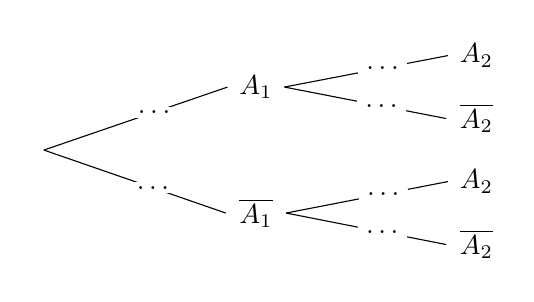
\begin{tikzpicture}[xscale=1,yscale=1,baseline={(R.base)}]
			
			\tikzstyle{noeud}=[fill=white,circle,inner sep=2pt]
			\tikzstyle{feuille}=[fill=white,circle,inner sep=2pt]
			\tikzstyle{etiquette}=[pos=0.6,fill=white, inner xsep=3pt, inner ysep=1.5pt]
			
			\def\DistanceInterNiveaux{2.8}
			\def\DistanceInterFeuilles{0.8}
			
			\def\NiveauA{(0)*\DistanceInterNiveaux}
			\def\NiveauB{(1)*\DistanceInterNiveaux}
			\def\NiveauC{(2)*\DistanceInterNiveaux}
			\def\InterFeuilles{(-1)*\DistanceInterFeuilles}
			
			\node[noeud] (R) at ({\NiveauA},{(1.5)*\InterFeuilles}) {};
			\node[noeud] (Ra) at ({\NiveauB},{(0.5)*\InterFeuilles}) {$A_1$};
			\node[feuille] (Raa) at ({\NiveauC},{(0)*\InterFeuilles}) {$A_2$};
			\node[feuille] (Rab) at ({\NiveauC},{(1)*\InterFeuilles}) {$\overline{A_2}$};
			\node[noeud] (Rb) at ({\NiveauB},{(2.5)*\InterFeuilles}) {$\overline{A_1}$};
			\node[feuille] (Rba) at ({\NiveauC},{(2)*\InterFeuilles}) {$A_2$};
			\node[feuille] (Rbb) at ({\NiveauC},{(3)*\InterFeuilles}) {$\overline{A_2}$};
			
			\draw (R.east)--(Ra.west) node[etiquette] {$\dots$};
			\draw (Ra.east)--(Raa.west) node[etiquette] {$\dots$};
			\draw (Ra.east)--(Rab.west) node[etiquette] {$\dots$};
			\draw (R.east)--(Rb.west) node[etiquette] {$\dots$};
			\draw (Rb.east)--(Rba.west) node[etiquette] {$\dots$};
			\draw (Rb.east)--(Rbb.west) node[etiquette] {$\dots$};
		\end{tikzpicture}

	\subsection*{Partie B}
		Pour vérifier le bon fonctionnement d'un relai, des tests indépendants les uns des autres sont effectués.

		Un test est positif si la présence d'au moins une erreur est détectée.

		On admet que la probabilité qu'un test soit positif est égale à 0,04.

		On choisit au hasard un échantillon de 50 tests réalisés sur le relai.

		Le nombre de tests réalisés est suffisamment grand pour assimiler ce choix à un tirage avec remise.

		\begin{enumerate}
			\item On note $X$ la variable aléatoire qui à chaque échantillon de 50 tests associe le nombre de tests positifs.

			Ainsi la variable aléatoire $X$ suit la loi binomiale de paramètres $n=50$ et $p=0,04$.

			\begin{enumerate}
				\item Déterminer la probabilité que 4 tests soient positifs dans cet échantillon.

				On arrondira le résultat à $10^{-2}$.

				\item Donner la probabilité qu'au moins un test soit positif dans cet échantillon.

				On arrondira le résultat à $10^{-2}$.
				\item Calculer l'espérance et la variance de la variable aléatoire $X$.
			\end{enumerate}

			\item On étudie une chaîne de transmission de l'information composée de 25 relais.

			On considère la variable aléatoire $X_{1}$ qui à chaque échantillon de 50 tests pratiqués sur le relai 1 associe le nombre de tests positifs.

			On définit de la même manière les variables aléatoires $X_{2}$ pour le relai $2$, \ldots, $X_{25}$ pour le relai 25.

			On admet que ces 25 variables aléatoires sont indépendantes entre elles et qu'elles admettent la même espérance égale à 2 et la même variance égale à 1,92.

			On note $M$ la variable aléatoire donnant la moyenne du nombre de tests positifs lors des contrôles effectués sur les 25 relais.

			On a donc \quad $M=\dfrac{X_{1}+X_{2}+\cdots+X_{25}}{25}$.
			\begin{enumerate}
				\item Vérifier que $\mathrm{E}(M)=2$ et montrer que $\mathrm{V}(M)=\np{0,0768}$.

				\item À l'aide de l'inégalité de Bienaymé-Tchebychev, montrer que la probabilité que la moyenne des tests positifs soit strictement inférieure à 7 est supérieure à 0,99.

				Indication : on pourra utiliser, sans justification, le fait que :
				\[P(M<7)=P(-3<M<7).\]
			\end{enumerate}
		\end{enumerate}

	\subsection*{Partie C}
		On désigne par $n$ un entier naturel non nul.

		On s'intéresse à une chaîne de transmission de l'information composée de $n$ relais.

		On considère l'évènement $A_{n}$ : \og le message reçu par le $n$-ième relai est sans erreur \fg{}.

		On note $p_{n}$ la probabilité que le message reçu au $n$-ième relai soit sans erreur.

		On a ainsi $p_{n}=P\left(A_{n}\right)$ et $p_{1}=0,96$.

		On admet que pour tout entier naturel $n \geqslant 1$,
		\[p_{n+1}=0,59 p_{n}+0,35.\]

		\begin{enumerate}
			\item Montrer par récurrence que pour tout entier naturel $n \geqslant 1$, \quad $p_{n+1} \leqslant p_{n}$.

			\item Montrer que la suite $(p_{n})$ est convergente.

			\item Déterminer la valeur exacte de sa limite.
		\end{enumerate}
